\documentclass[twoside,numberorder]{zjuthesis}
%==============================================================
%==============================================================

%自己需要增加什么 package 或修改什么设置的话,都放在这里吧。
\usepackage{url}
\usepackage{pdfpages} %插入pdf文件
\usepackage{float}% 插入图形中使用H
\usepackage{subfigure}
\usepackage{enumerate} %自定义编号样式
%设置图片caption字体
\captionsetup{font={scriptsize}}
\setcounter{tocdepth}{2} %设置目录级数到subsection

\usepackage{pythonhighlight}
\usepackage{minted}
\usepackage{xcolor}



%一些全局工具的定义
\DeclareMathOperator*{\argmin}{arg\,min}
\DeclareMathOperator*{\argmax}{arg\,max}

%==============================================================
%==============================================================
\begin{document}

%==============================================================
%==============================================================
%这部分是论文封面、题名页需要的信息,请根据《研究生学位论文编写规则》自行修改

  %论文题目:{中文}{英文}
  \zjutitle{BPA电网模型导入DIgSILENT的研究和开发}%
           {Transform of power grid models from BPA to DigSILENT}
  %作者:{中文姓名}{英文}{学号}
  \zjuauthor{孙竞凡}{Jingfan Sun}{3110104734}
  %指导教师:{导师中文名}{导师英文名}
  \zjumentor{甘德强}{Deqiang Gan}
  %个人信息:{年级}{专业名称}
  \zjuinfo{}{电气工程及其自动化1101}
  %学院信息:{学院中文}{学院英文}{subject}
  \zjucollege{电气工程学院}{College of Electrical Engineering}{Machine Learning}
  %日期:{Submitted Date}
  \zjudate{June 1, 2015}

%==============================================================
% 这部分除了“取舍”外,不需要自己修改,必要信息都已在上面设置。

  %封面
  %%============================================================
%% 中文封面

\thispagestyle{empty}

\vspace{5mm}

\begin{center}
   
\includegraphics[width=108mm]{images/zjdx}
\end{center}

\centerline{\songti\erhao\textbf{本科生毕业论文(设计)}}

\vspace{4mm}

\begin{center}
  
\includegraphics[width=35mm]{images/standxb}
\end{center}

\vspace{25mm}

{\hspace{16mm}\songti\sanhao\bfseries 题目:
  \hspace{2mm} \begin{minipage}[t]{98mm}\linespread{1.1}\uline{\zjutitlec}\end{minipage}}

\vspace{7mm}

\begin{tabbing}
    \hspace{30mm} \songti\sihao 姓 \hspace{-2.7mm} \= \songti\sihao 名与学号: \= \underline{\makebox[6cm]{\sihao\zjuauthornamec\hspace{3mm}\zjuauthorid}} \\[2mm]
              \> \songti\sihao 指导教师: \> \underline{\makebox[6cm]{\sihao\zjumentorc}} \\[2mm]
              \hspace{30mm} \songti\sihao 年 \hspace{-2.7mm} \= \songti\sihao 级与专业: \= \underline{\makebox[6cm]{\sihao\zjugrade\hspace{3mm}\zjumajor}} \\[2mm]
              \> \songti\sihao 所在学院: \> \underline{\makebox[6cm]{\sihao\zjucollegec}}
\end{tabbing}


%%============================================================
% empty page for two-page print
\ifthenelse{\equal{\zjuside}{T}}{%
  \newpage\mbox{}%
  \thispagestyle{empty}}{}

%%============================================================
%% English Cover
\newpage
\thispagestyle{empty}

\vspace{5mm}

\begin{center}
    \songti\xiaoyi A Dissertation Submitted to Zhejiang University for the Degree of Bachelor of Engineering
\end{center}

\vspace{4mm}

\begin{center}
  
\includegraphics[width=35mm]{images/standxb}
\end{center}

\vspace{25mm}

{\hspace{3mm}\songti\sanhao\bfseries TITLE:\hspace{4mm}\begin{minipage}[t]{124mm}\linespread{1.1}{\renewcommand\baselinestretch{0.9}\selectfont\uline{\zjutitlee}\par}\end{minipage}}

\vspace{7mm}

\begin{tabbing}
    \hspace{18mm} \= \sanhao Author:\hspace{19mm} \= \underline{\makebox[8cm]{\sanhao\zjuauthornamee\hspace{3mm}\zjuauthorid}} \\[2mm]
                  \> \sanhao Supervisor: \> \underline{\makebox[8cm]{\sanhao\zjumentore}} \\[2mm]
                  \> \sanhao Subject: \> \underline{\makebox[8cm]{\sanhao\zjusubject}} \\[2mm]
                  \> \sanhao College: \> \underline{\makebox[8cm]{\sanhao\zjucollegee}} \\[2mm]
                  \> \sanhao Submitted Date: \> \underline{\makebox[8cm]{\sanhao\zjusubmitteddatee}}
\end{tabbing}

%%============================================================
% empty page for two-page print
\ifthenelse{\equal{\zjuside}{T}}{%
  \newpage\mbox{}%
  \thispagestyle{empty}}{}

  %诚信承诺书
  %% 诚信承诺书

\newpage
\thispagestyle{empty}

\begin{center}
\heiti\xiaosan 浙江大学本科生毕业论文(设计)诚信承诺书
\end{center}

\vspace{5mm}

{\songti\sihao
\begin{enumerate}
  \item 本人郑重地承诺所呈交的毕业论文(设计),是在指导教师的指导下严格按照学校和学院有关规定完成的。
  \item 本人在毕业论文(设计)中引用他人的观点和参考资料均加以注释和说明。
  \item 本人承诺在毕业论文(设计)选题和研究内容过程中没有抄袭他人研究成果和伪造相关数据等行为。
  \item 在毕业论文(设计)中对侵犯任何方面知识产权的行为,由本人承担相应的法律责任。
\end{enumerate}

\vspace{12mm}
\hspace{20mm}毕业论文(设计)作者签名:
\begin{flushright}
    \underline{\hspace{4em}} 年 \underline{\hspace{2em}} 月 \underline{\hspace{2em}} 日
\end{flushright}}

\ifthenelse{\equal{\zjuside}{T}}{%
  \newpage\mbox{}%
  \thispagestyle{empty}}{}


  \frontmatter   
  \pagenumbering{Roman}

  %中文摘要
%  %% 中文摘要
\chapter*{\centerline{摘\quad 要}}
\chaptermark{摘要}
\addcontentsline{toc}{chapter}{摘要}

\vspace{1em}
大多数机器学习的算法都可以看作是寻找一个函数或模型$f$让它的经验误差达到最小。
但是这只有在你有足够多的训练数据的时候才能工作得很好。现在人们逐渐开始关注训练
数据稀少时的学习问题,正则化就显得越来越重要了。通过在原始的目标函数中加入一个
额外的正则化项,我们可以对解空间进行限制,从而实现增加算法的泛化性能。不过,现在
的大多数正则化的技术都没有专门考虑时间正则化的问题。考虑到现在有大量的会随着时间
而逐步发展的数据(例如动态的web页面、博客内容以及股票价格等),我们提出一个新
的正则化方法,同时考虑数据在时间和空间上的平滑性质。我们把这个新的正则化方法应用
到视频压缩里,实验结果展示了这种算法的效力。

\vspace{1em}

\noindent\textbf{关键词}:\quad 机器学习,正则化,视频压缩

  %英文摘要
%  %% 英文摘要
\chapter*{\centerline{Abstract}}
\chaptermark{Abstract}
\addcontentsline{toc}{chapter}{Abstract}

\vspace{1em}
In order to achieve the automatic import of BPA data into DIgSILENT, I analyzed mathematical models in equipments in BPA and DIgSILENT, and got the two conversion formulas between device model parameters. I studied the functional and technical characteristics of DIgSILENT Python Module and summarized the work steps to convert BPA grid model into DIgSILENT. I determined the use of Python scripting language to design the programs for converting BPA grid model into DIgSILENT and developed to achieve the program. Finally, I tested the program with IEEE9 node examples and IEEE39 node examples respectively. It is proved that the program meets the design requirements.

\vspace{1em}

\noindent\textbf{Keywords}:BPA,DIgSILENT,data convert


%==============================================================
%这部分不需要自己修改。

  %目次页
  \tableofcontents
  \chaptermark{目录}
  \addcontentsline{toc}{chapter}{目录}
  

  \mainmatter

%==============================================================
  
  %文献综述
  \chapter{文献综述}

\section{概述}

\subsection{项目研究背景}

作为一个具有时变性的大型复杂系统,电力系统在国名经济和生活中扮演着至关重要的角色。在进行电力系统的规划、设计、运行和维护时,为了保证其可靠、安全地运行,需要准确地考察电力系统的动态特性和静态特性,需要有一个强有力的工具来分析实际电力系统的运行情况。然而电力系统的特点决定了难以采用试验的方法来实现,必须采用仿真的手段,仿真可以分为物理仿真和数字仿真。随着计算机和数值计算技术的迅猛发展,电力系统数字仿真技术得到了飞速发展,并以其良好的经济性和便利性成为分析、研究电力系统的必要工具。目前电力系统数字仿真不仅为电力系统的规划、设计提供了基础,而且为电力系统调度、运行的安全性和可靠性等方面提供了依据。

电力系统仿真软件以数学模型代替实际电力系统,用数值方法对系统的运行特性进行试验和研究,它已经成为电力系统研究人员不可缺少的有力工具。在电力系统的规划、设计和运行中,电力系统仿真软件可以用来确定规划方案、拟定运行方式、整定自动装置的控制参数、进行事故分析和辅助运行人员做出正确的决策,大大提高电网的运行效率。

电力系统的发展也为电力系统数字仿真提出了更高的要求,采用单一的电力仿真软件对大电网进行仿真已经不足以满足实际研究的需要。这主要体现在以下几个方面:第一,不同软件采用的系统元件数学模型或者数字仿真数值计算方法可能不同,在功能上也会有差异;第二:不同的软件在计算规模上有差别;第三:由于新型电力元件的不断出现,某些软件在元件模型库上可能存在不足,软件不允许用户自定义模型等等。因此在对大规模电力系统进行仿真时需要综合比较以选择适当的仿真工具。

\subsection{项目发展历史、现状和趋势}

电力系统仿真软件的开发研究起源于上世纪五、六十年代,受到当时的计算机价格、内存容量和计算速度等多方面的严重限制。八十年代以来,随着计算机软件和硬件的高速发展,先进数学计算方法的引入,电力系统仿真软件取得了长足的进步,功能日益强大,计算效率大大提高,使用也更加方便灵活。目前,国际上有多种电力系统仿真软件,在世界上不同国家和地区的各级电力企业、研究所和高校中得到了较为广泛的应用,对各国电力系统的实践和研究发挥了很大的作用。我国电力系统仿真软件的开发和研究也起步较早,在上世纪七十年代有较大的发展。

目前,国内的电力科研单位一般都有一种或者几种电力系统仿真软件,其中最为普遍的是 BPA 和 PSASP 软件,国内电网数据文件也普遍采用这两种软件的数据格式。在利用其它软件进行计算时,如何运用已有的数据文件,准确快速的进行新数据的整理和输入,是研究人员经常遇到的问题。对于一个小系统,手工填写数据是可行的,但是对于大规模的系统,如果以人工方式填写数据,不仅需要耗费大量的人力和物力,并且出现错误的可能性也会增加。由于电力系统的数据文件都是基于系统的物理模型,有很多共同的属性,所以通过编写数据转换程序对这些仿真软件的数据格式进行自动转换是可行的,也是必要的。

随着电网规模的不断增大,仿真软件也在不断的提升。它们的运行规模在不断扩大,运行速度不断提升,功能不断增加,精度不断提高,元件模型与实际越来越贴近,各个仿真软件在不同方面的优缺点也愈见明显,所以需要建立一个统一的数据库。

早期的电力系统仿真软件实际上是一个程序包,针对不同的分析功能需要采用相应的计算程序并调用相应格式的数据,这使得用户操作起来极为繁琐,而且也增加了出错几率。新一代的分析软件打破了这种传统模式,在将各种计算功能集成在一个统一的软件平台的同时,引入了数据库的观念,将不同计算过程所要调用的数据统一存放在一个分级的面向对象的数据库中。这样,用户就不再像往常一样,需要编辑、组织和维护众多不同类型的文件以及其中所包含的数据。软件通过一个有效的数据管理器,将用户和内建数据库连接起来。

\section{项目的研究意义}

电力系统在国民经济中有着非常重要的作用,随着电力系统技术的发展,针对大型电力系统的仿真计算不仅为电力系统的规划,而且为电力系统的计划、调度、运行的安全性与可靠性等方面,都提供了强大的技术支持,电力系统无法离开仿真这个工具已是不争的事实。电力系统规划的方案是靠仿真得到的;新元件的接入、运行方式的确定是用仿真结果作为依据的;新方法研究、新装置设计、参数确定是用仿真来确认的。电力系统仿真软件已经成为电力系统研究、计算、运行的有力工具。

由于电力系统仿真软件是指导电力系统运行、规划和决策的最基本工具,所以,一般网省局都规定:对新引进的程序必须与现有程序进行认真的比较,证明其结果一致,方可在实际电网中推广应用。

与此同时,采用单一的电力仿真软件对大电网进行仿真已经不足以满足实际研究的需要。这主要体现在以下几个方面:第一,不同软件采用的系统元件数学模型或者数字仿真数值计算方法可能不同,在功能上也会有差异,比如电力系统常用的数据格式是基于BPA文本文件,其缺陷是不易于实现自定义等高级操作,随着大规模新能源接入后其更新速度赶不上科研需要,PSS/E自定义功能强大,易于实现自定义等功能,但其缺陷是难以实现电磁暂态仿真,只能实现三相对称的机电暂态仿真,DIgSILENT功能更为强大,但在大规模计算时的速度不能和PSS/E媲美;第二:不同的软件在计算规模上有差别,后文中也将会提及;第三:由于新型电力元件的不断出现,某些软件在元件模型库上可能存在不足,软件不允许用户自定义模型等等。因此,在对大规模电力系统进行仿真时需要综合比较以选择适当的仿真工具。

对于不同软件间的数据转换,针对简单的网络,手动的模型转换和仿真验证还是可以接受的。但是如果面临较大的网络,手动的转换是十分耗费人力和时间的。然而,现有的分析软件或多或少都存在数据兼容的问题:即不同的软件开发商定义了不同的数据格式,而这些数据格式不被其它软件所识别。虽然有些软件自带了一些数据格式的转换程序,但其功能只限于少数软件间的格式转换,对某些具体情况并不适用。例如,PSS/E这种在国际上有着众多用户的软件并且针对国际上常用的数据格式也有数据转换接口程序,但是DIgSILENT针对PSS/E的数据的转换程序做的并不好,只能实现比较简单数据的转换。而对于BPA到DIgSILENT的数据转化软件更是如此,现在还没有现成的两者间的数据转换程序。因此,需要开发第三方提供的数据接口程序。

\section{该项目的国内进展情况}

对于BPA和DIgSILENT之间的数据导入问题,刘庆等学者[1]进行了研究,他们首先分析了 BPA 和 DIgSILENT 的数学模型,得到了转换公式,用来完成两种仿真软件一次设备模型之间的参数转换,接着通过DIgSILENT 的DPL 语言和 DGS 接口,结合 VC6 和 DPL 实现方案,设计了软件的整体结构,用于将 BPA 模型参数自动导入到 DIgSILENT 中。文献[2]综合比较了当前主要使用的各种电力系统仿真软件的功能特点和应用情况,分析了各自的优势。文献[4]总结了我国常用的电力系统仿真软件,以及其现状和发展趋势,并编写了DIgSlLENT与仿真软件PSS/E以及PSASP之间的数据转换程序。文献[3]集中介绍了DIgSlLENT在电力系统应用方面的主要功能和特点。文献[5], [6]对BPA常用的潮流数据卡进行了分
析,得到了BPA 与 PSS/E 模型的区别和相应的转换关系,并使用C++完成了数据转换程序。文献[7]介绍了DIgSILENT软件的详细功能。

国内已有很多学者使用DIgSlLENT建模仿真,分析电网数据,为决策提供依据,文献[8]-[10]均选择DIgSlLENT作为仿真平台,研究风电站并网的运行和控制。

\section{项目研究的主要内容}

本项目基于DIgSILENT平台,致力于研究从BPA到DIgSILENT的数据转换问题:将BPA的数据导入DIgSILENT中,利用Python语言编程,实现从外部数据的读取,并且将读到的数据在DIgSILENT中建立相应的模型并予以赋值,从而在DIgSILENT得到与BPA中相同的数据模型,进而可以利用两个软件不同的优势进行数据的计算。
论文的工作主要从以下几个方面展开:
\begin{itemize}
\item 对DIgSILENT和BPA数据的介绍。分别对DIgSILENT和BPA的数据特点进行具体的介绍,包括发电机模型,负荷模型等在两个不同软件的不同特点。
\item 从DIgSILENT里找到BPA软件中数据对应的模型及其参数位置。
\item 用Python语言进行编程,将外部数据所代表的模型意义完全的在DIgSILENT中重现出来,即在DIgSILENT中重新建立模型,并赋予响应的参数值。建立他们之间的关系。
\end{itemize}

\begin{thebibliography}{99} % Bibliography - this is intentionally simple in this template

\bibitem{1}刘庆, 张东英, 刘燕华, 等. BPA 电网模型自动导入 DIgSILENT 的研究和开发[J]. 电力系统保护与控制, 2014, 42(16): 112-117.

\bibitem{2}李广凯, 李庚银. 电力系统仿真软件综述[J]. 电气电子教学学报, 2005, 27(3): 61-65.

\bibitem{3}吕涛, 韩祯祥. 电力系统仿真软件 DIgSILENT 介绍[J]. 华东电力, 2005, 32(12): 37-41.

\bibitem{4}吕涛. 电力系统仿真软件的运用与比较[M]. 浙江大学, 2005.

\bibitem{5}马龙义. BPA与PSS/E仿真模型分析与转换研究[D]. 华南理工大学, 2010.

\bibitem{6}马龙义, 武志刚, 侯冠基, 等. BPA 与 PSS/E 的暂稳态模型比较和数据转换[J]. 电力系统及其自动化学报, 2010, 22(5): 128-134.

\bibitem{7}PowerFactory. User's Manual DIgSILENT PowerFactory. Version 14.0 DIgSILENT GmbH. Gomaringen, Germany July 2010. Publisher: DIgSILENT GmbH. 

\bibitem{8}李东东, 王凯凯, 叶辰升. 采用双馈机组的风电场无功功率控制研究[J]. 电力系统保护与控制, 2013, 41(13): 37-42.

\bibitem{9}付超, 朱凌, 王慧, 等. 风电场并网在线预警系统研究[J]. 电力系统保护与控制, 2011, 39(17): 64-69.

\bibitem{10}苑国锋, 李永东, 柴建云, 等. 1.5 MW 变速恒频双馈风力发电机组励磁控制系统试验研究[J]. 电工技术学报, 2009, 24(2): 42-47.

\end{thebibliography}

  %外文文献翻译
  \chapter{外文文献翻译}
%==============================================================
%英文文献
  \section{外文文献原稿}

  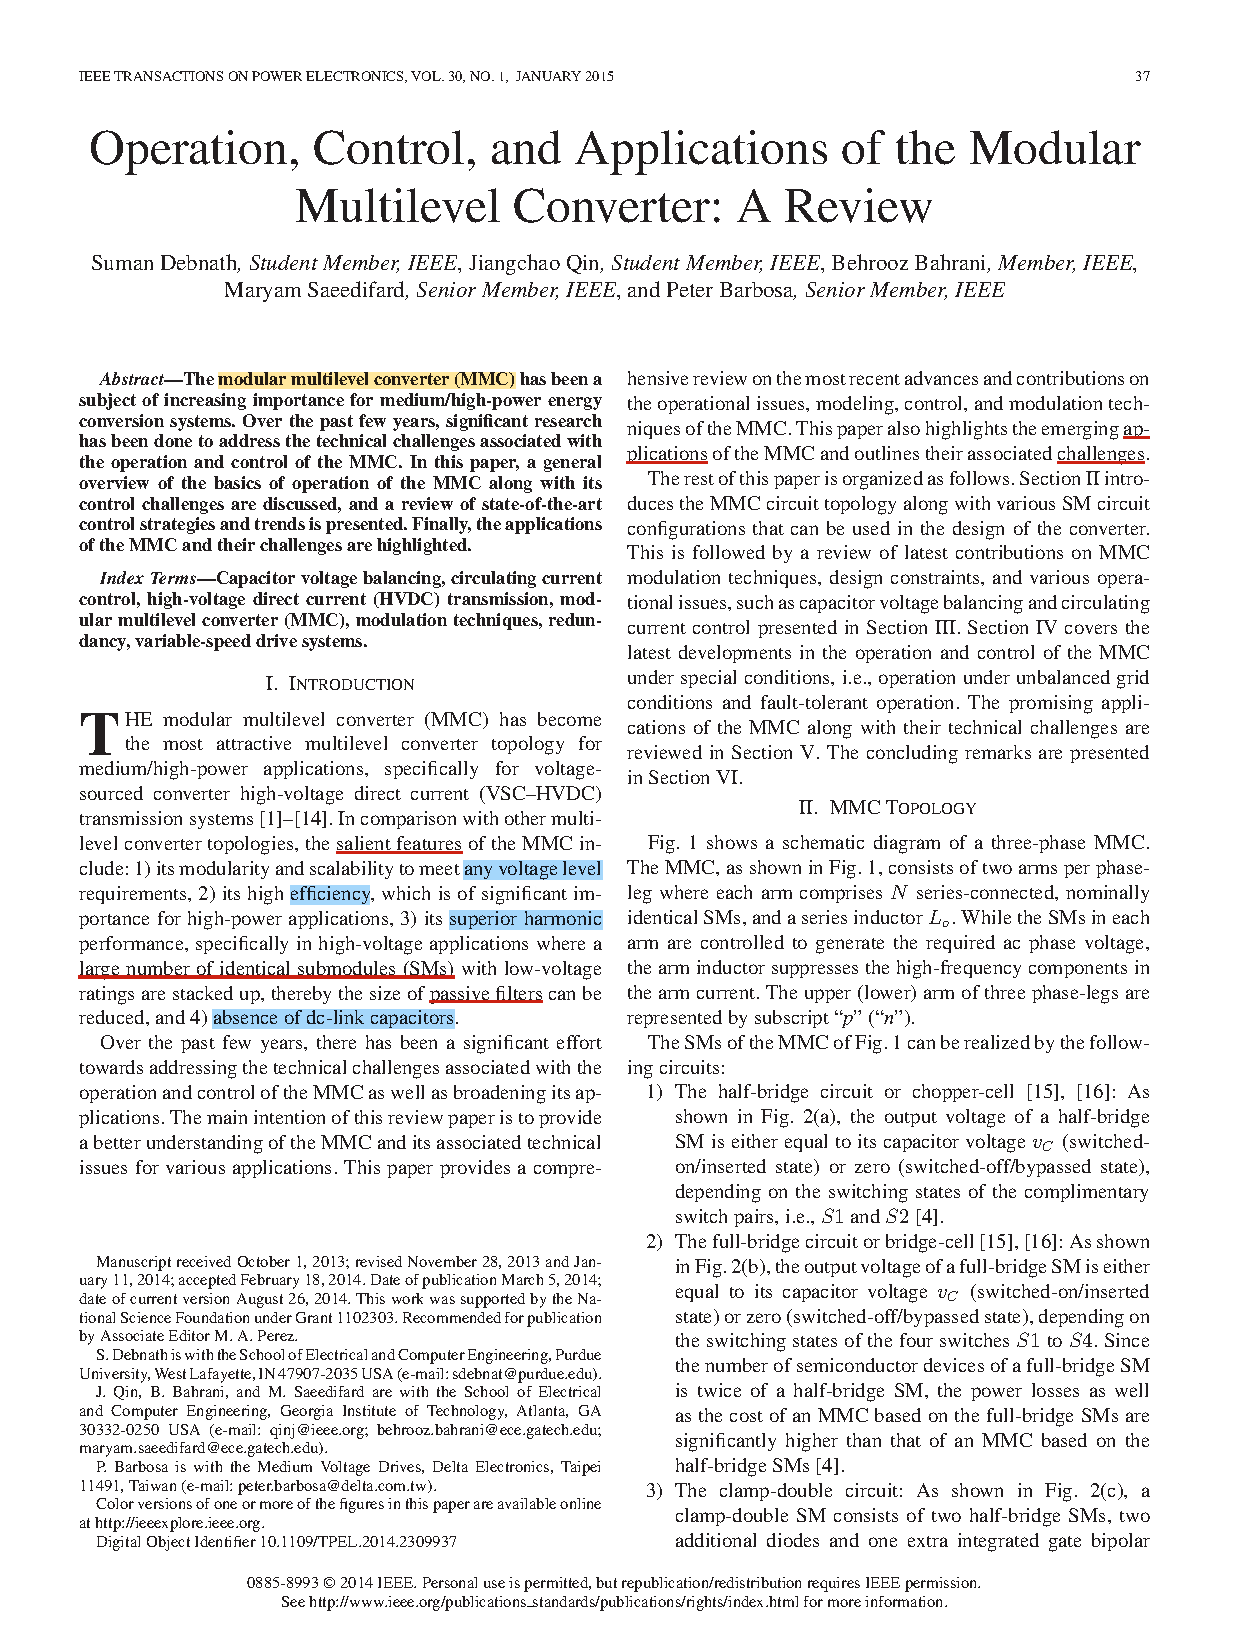
\includepdf[pages={1-17}]{data/Paper.pdf}

%==============================================================
  \section{中文翻译译稿}
  
  模块化多电平换流器的运行、控制和应用
  
  \textbf{摘要:}\quad  模块化多电平换流器(MMC)对于中高压电力换流系统来说正在变成一个越来越重要的课题。在过去的几年里,重要的研究指出了伴随着MMC运行和控制所产生的技术挑战。在这篇文章里,我们综述了MMC运行基础并讨论了控制所面临的挑战和先进的控制策略和趋势。最后,强调了MMC的应用和挑战。
  
  \textbf{关键词:}\quad 电容电压平衡,环流控制,高压直流{HVDC}输电,模块化多电平换流器{MMC},模块化技术,冗余,变速传动系统
  
  \subsection{导言}
  
  模块化多电平换流器(MMC)正成为中高级电压应用中最有吸引力的多电平换流器拓扑,特别是对电压源换流器高压直流输电系统。和其他多电平换流器拓扑相比,MMC的显著特点包括:1)、模块化和可测量性满足任何电压等级需要;2)、高效,对高压应用有特别重要性;3)、优秀的谐波表现,特别是在高压应用当中,在这种应用中通过组合大量相同的低压子模块,减小了被动滤波器的大小;4)、不需要直流连接电容。
  
  在过去几年中,有大量的研究致力于找到MMC控制和运行所带来的技术挑战并扩展其应用。这篇综述的主要目的是为MMC提供一个更好的理解和针对各种应用的技术命题。这篇文章全面总结了关于MMC运行、建模、控制和模块化技术最近的成果,同时强调了MMC的广泛应用和伴随的挑战。
  
  文章的其余部分按如下方式展开。第二部分介绍MMC电路拓扑和能应用于换流器设计的各种子模块。接下来是关于MMC模块化技术、设计局限和各种运行问题最新成果的综述,包括电容器电压平衡和环路电流控制都在第三章中呈现。第四章包括MMC在特殊环境下运行和控制的最新发展,例如不平衡电网条件下的运行和容错运行。第五章介绍MMC的广泛应用和随之而来的技术挑战。第六章总结了全文。
  
  \subsection{MMC拓扑}
  
\begin{figure}[h]
\begin{minipage}[t]{0.5\linewidth}
\centering
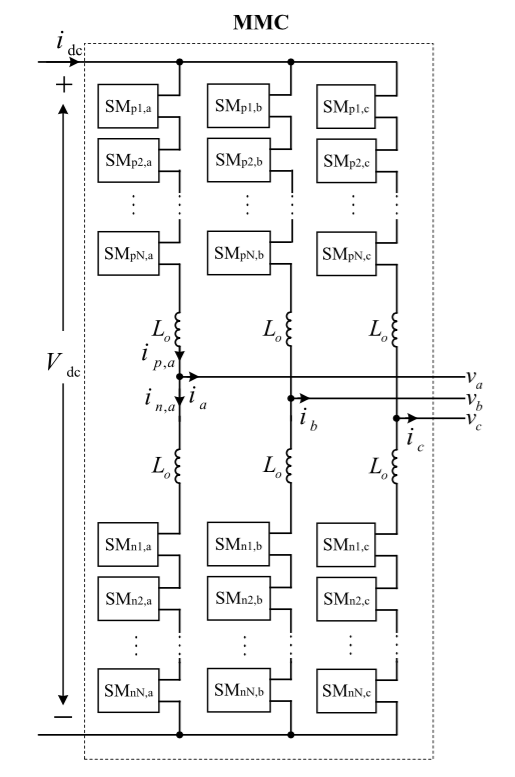
\includegraphics[width=3.2in]{images/Paper_Fig_1.png}
\setcaptionwidth{2.5in}
\caption{MMC示意图}
\end{minipage}%
\begin{minipage}[t]{0.5\linewidth}
\centering
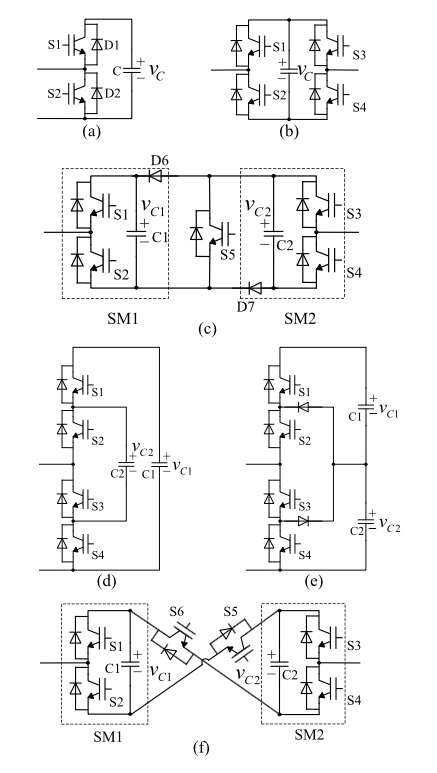
\includegraphics[width=3.2in]{images/Paper_Fig_2.png}
\setcaptionwidth{2.5in}
\caption{ 不同SM拓扑:\quad(a)半桥\quad(b)全桥\quad(c)双钳制\quad(d)三级FC\quad(e)三级NPC和(f)五级跨接SM}
\end{minipage}
\end{figure}
  
  图3.1所示是三相MMC的示意图,这个MMC由每相两臂组成,每臂由$N$个序列连接、名义上独立的SM和一个序列电感$L_0$组成。尽管控制每一臂中的SM长生需要的交流相电压,臂电感器抑制了臂电流中的高频分量。三相臂中的上(下)臂表示成$"p"("n")$。
  
  图3.1中MMC的SM可以从如下回路来理解:
  \begin{enumerate}[1)]
  \item 半桥回路或斩波单元(chopper-cell):如图3.2(a)所示,半桥SM的输出电压或等于其电容电压$v_c$(开/接入状态),或等于$0$(关/旁路状态),取决于开关对的开关状态,例如$S1$和$S2$。
  \item 全桥回路或桥臂单元(bridge-cell):如图3.2(b)所示,全桥SM的输出电压或等于其电容电压$v_c$(开/接入状态),或等于$0$(关/旁路状态),取决于四个开关$S1$到$S4$的状态。因为全桥SM的半导体数是半桥SM半导体数的两倍,基于全桥SM的MMC的能耗和费用都高于基于半桥SM的MMC。
  \item 双钳制回路(clamp-double):如图3.2(c)所示,双钳制回路SM由两个半桥SM、两个额外的二极管和一个与有反向二极管并联的绝缘栅双极型晶体管(IGBT)组成,正常操作中,开关$S5$一直开启,双钳制回路SM等价于两个串联的半桥SM,与同电压等级数量的半桥和全桥MMC相比,双钳制回路MMC的半导体能耗比半桥MMC高但比全桥MMC少。
  \item 三级换流器回路:如图3.2(d)和(e)所示,三级SM由三级中性点钳制(neutral-point-clamped: NPC)或三级飞跨电容(flying capacitor: FC)换流器。三级FC MMC和半桥MMC半导体能耗相同。相比之下,三级NPC MMC的半导体能耗比半桥MMC高但比全桥MMC低。从制造和控制的角度,这种SM回路吸引力不大。
  \item 五级跨接回路(cross-connected):如图3.2(f)所示,一个五级跨接回路由两个半桥SM背靠背连接两个有反向并联二极管的IGBT组成。它的半导体能耗与双钳制回路相同。
  \end{enumerate}
  
  表3.1展示了有关不同SM回路电压等级、直流侧短路容错能力和电能损耗的比较。直流侧短路问题是MMC-HVDC系统的主要挑战之一,这部分会在第五章A中讨论。在这所有SM回路中,半桥SM是适用于MMC最受欢迎的SM。因为其中只有两个开关器件,所以减少了元件数并且提高了效率。在此之后,基于半桥SM的MMC开始被人们关注。需要注意的是,只有很少的换流器结构源自MMC拓扑。本文着重讨论图3.1所示的称为双星(double-star)的MMC结构。
  
\begin{table}[h]
\centering
\begin{tabular}{cccc}
\toprule
SM回路 & 电压等级 & 直流容错 & 能耗\\
\midrule
半桥 & $0, v_c$ & 否 & 低 \\ 
全桥 & $0, +v_c$ & 是 & 高 \\ 
双钳制 & $0, v_{C1}, v_{C2}, (v_{C1} + v_{C2})$ & 是 & 中 \\ 
三级FC & $0, v_{C1}, v_{C2}, (v_{C1} - v_{C2})$ & 否 & 低 \\ 
三级NPC & $0, v_{C2}, (v_{C1} + v_{C2})$ & 否 & 中 \\ 
五级跨接 & $0, v_{C1}, v_{C2}, +(v_{C1} + v_{C2})$ & 是 & 中 \\ 
\bottomrule
\end{tabular}
\caption{不同SM回路比较}
\end{table}
  
  \subsection{MMC的模块化、设计、控制和建模}
  
  \subsubsection{模块化技术}
  
  针对MMC开发/提出的基于单个参考波形的不同的脉宽调制(PWM)技术包括:
  %%%%%%%%%%%%%%%%%%%%%%%%%%%%%%%%%%
  \begin{enumerate}[1)]
  \item 载波层叠PWM技术(CD-PWM):这种技术需要$N$个独立三角载波波形关于$0$坐标轴对称出现。相电压参考波形和载波的比较产生了所需的开关输出相电压等级。对应于三角形载波的电压变换由一个特定SM的开启/旁路状态决定。基于载波波形的相变换,这一技术被进一步划分为:a)同相层叠(PD);b)正负反向层叠(POD);c)交替反向层叠(APOD),分别如图3.3(a)-(c)所示。使用这些技术的不足之处包括SM电容上电压波动的不等分布和大量环流。为了提高交流侧电压的谐波失真,使用简单载波旋转技术、修正载波旋转技术或信号旋转技术来所有SM电容器的电压平衡。尽管采用了SM电容器电压平衡技术,输出电压有一个相对较高的总谐波失真(THD)。为了提高这些技术的表现,提出了一种有关SM电容电压平衡技术的PD PWM技术。在这种基于PD载波波形的技术中,有关三角形载波的电压变换不再针对某个特定的SM。在这种技术中,参考波形和载波波形的比较产生出$(N+1)-level$波形,进而分别决定了插入上下桥臂中SM的数量。取决于桥臂中的电流方向河SM电容器的电压状态,在上(下)桥臂中插入除$N$个SM之外特定数量的SM来最小化SM电容器电压间的差异。Mei等人提出了一种带选择性回路偏置映射法的PD PWM技术来平衡SMSM电容器。这种方法实现了使用下列反馈的载波旋转:a)最大/最小SM电容电压和b)桥臂电流方向。这种技术的优点包括:a)不需要额外参考信号来控制SM电容器和b)即便在大量SM情况下易于用简单的现场可编程门阵列(FPGA)实现。
\begin{figure}[h]
\begin{minipage}[t]{0.5\linewidth}
\centering
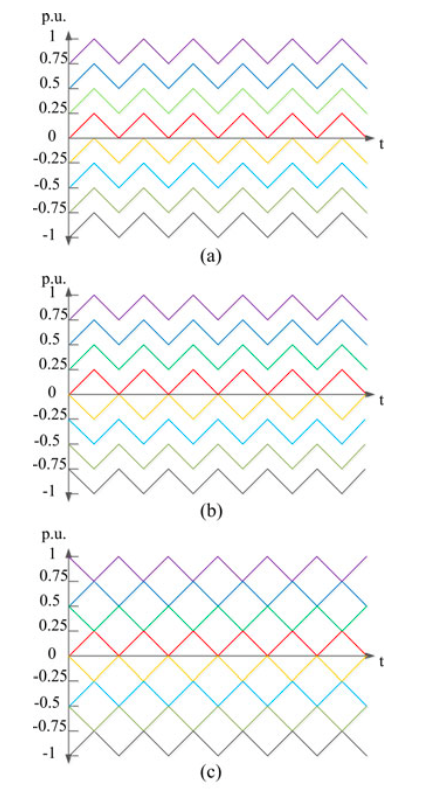
\includegraphics[width=3.2in]{images/Paper_Fig_3.png}
\end{minipage}
\begin{minipage}[t]{0.5\linewidth}
\centering
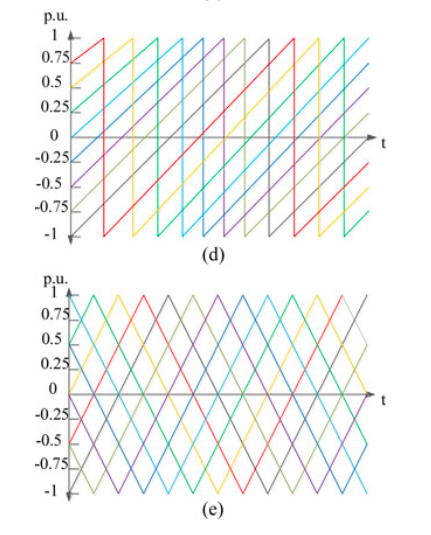
\includegraphics[width=3.2in]{images/Paper_Fig_4.png}
\end{minipage}
\setcaptionwidth{\linewidth}
\caption{多电平载波:\quad (a) PD, \quad (b) POD, \quad (c) APOD, \quad(d) saw-tooth, and (e) 相变换载波}
\end{figure}
  %%%%%%%%%%%%%%%%%%%%%
  \item 次谐波技术:在这种技术中,每相有$2N$个独立的载波,锯齿波或三角波,之间有$\theta=360^{\circ}/2N$相位差,如图3.3(d)和(e)所示。假设对PD PWM和次谐波技术有相同数量的开关变换,PD PWM技术产生更好地线到线电压THD。
  \end{enumerate}
  
  另外,基于使用多参考波形有几种模块化技术。这些模块化技术包括:
  \begin{enumerate}[1)]
  \item 直接模块化:在这种模块化技术中,$j$相的上下桥臂电压由两个互补的正弦参考曲线控制,如下所示:
\begin{align*}
n_{p,j,ref} &= N\frac{\frac{V_{dc}}{2}-v_{j,ref}}{V_{dc}}\tag{1a}\\
n_{p,j,ref} &= N\frac{\frac{V_{dc}}{2}+v_{j,ref}}{V_{dc}}\tag{1b}
\end{align*}
  其中$v_{j,ref}$代表参考输出电压,$n_{p,j,ref}$和$n_{n,j,ref}$是上下桥臂中开启SM数量的参考波形。(1)中的参考波形和PD载波波形比较,在$0$到$N$中波动,来决定上下桥臂中需要开启的SM数量。直接模块化技术的主要缺点在于存在环路电流,增加了换流器能耗和组件的额定值。
  \item 间接模块化:在这种技术中,$j$相上下桥臂的参考波形如下给出:
\begin{align*}
n_{p,j,ref} &= N\frac{\frac{V_{dc}}{2}-v_{j,ref}-v_{reg,j}^\Sigma-v_{reg,j}^{circ}}{\sum^N_{i=0}v_{cp,i,j}}\tag{2a}\\
n_{p,j,ref} &= N\frac{\frac{V_{dc}}{2}+v_{j,ref}-v_{reg,j}^\Sigma-v_{reg,j}^{circ}}{\sum^N_{i=0}v_{cn,i,j}}\tag{2b}
\end{align*}
  其中$v_{cx,i,j}$表示$j$相桥臂$x$中$SM-i$的电容电压,$v_{reg,j}^\Sigma$和$v_{reg,j}^{circ}$用来控制$j$相的总能量并分别平衡桥臂之间的能量。类似于直接模块化技术,参考波形和PD载波波形比较,在$0$到$N$中波动,来决定上下桥臂中需要开启的SM数量。这种技术可以进一步细分成:
  \begin{enumerate}[a)]
  \item 闭环控制:闭环控制中,(2)中的$\sum^N_{i=0}v_{cp,i,j}$项基于实际测量电容电压计算,进一步,$v_{reg,j}^\Sigma$和$v_{reg,j}^{circ}$从$j$相桥臂电容储存的闭环控制总能量和桥臂间能量平衡分别获得。每个桥臂间储存能量的平衡暂时取决于基频正弦环路电流。这种技术的优点在于i)平均SM电容电压的控制,使得能在高电压等级和低输出电压下运行,和ii)上下桥臂间能量平衡的控制。
  \item 开环控制:开环控制中,(2)中的$\sum^N_{i=0}v_{cp,i,j}$项基于估计测量电容电压计算。另外,$v_{reg,j}^\Sigma=0$并且估计$v_{reg,j}^{circ}$来降低环路电流的谐波并保证换流器的稳定控制。这种估计由求解描述换流器动态的方程获得,使用测量得到的输出电流和直流连接电压。这种技术的优点在于不需要电压传感器,控制简单迅速。尽管如此,主要缺点在于难以准确估计描述系统动态所需要的真实参数。
  \end{enumerate}
  %%%%%%%%%%%%%%%%%%%%
  \item 相变换载波PWM技术(PSC PWM):在这种技术中,MMC的每个SM独立控制,Sm的电压平衡任务分为平均控制和平衡控制。每一个SM上下桥臂中的的参考波形如下给出:
\begin{align*}
m_{p,i,j} &= N\frac{\frac{V_{dc}}{2}-\frac{v_{j,ref}}{N}+v_{a,j}+v_{b,i,j}}{v_{cp,i,j}}\tag{3a}\\
m_{p,i,j} &= N\frac{\frac{V_{dc}}{2}+\frac{v_{j,ref}}{N}+v_{a,j}+v_{b,i,j}}{v_{cn,i,j}}\tag{3b}
\end{align*}
  其中$v_{a,j}$和$v_{b,i,j}$分别是平均和平衡控制器输出。平均和平衡技术分别控制每一相桥的平均SM电容器电压。每一个SM电压参考波形和三角载波的比较产生相应SM的开关信号。每一个桥臂的三角形载波波形基于次谐波技术实现。这项技术的主要缺点在于随着SM数量的增加实现难度加大并且在特定运行情况下存在不稳定性。通过基于上下桥臂中电容电压的不同在参考电压中引入另一个概念,桥臂平衡控制,可以改善后一种缺点。
  \end{enumerate}
  %%%%%%%%%%%%%%%%%%%%%%%%%%%%%%%%%%
\begin{table}[h]
\begin{center}
\small
\begin{tabular}[c]{ccccc}
\toprule
性质 & 改进PD-PWM & 直接模块化 & 间接模块化 & PSC-PWM\\
\midrule
参考波形数 & $1$ & $2$ & $2$ & $2N$\\ 
稳定所需额外控制器数 & 否 & 否 & 是 & 是\\ 
是否存在环路电流 & 是 & 是 & 否 & 否 \\ 
实现难度 & 中 & 中 & 低(开环)-中(闭环) & 高(随着$N\uparrow$) \\ 
\bottomrule
\end{tabular}
\caption{模块化策略比较}
\end{center}
\end{table}
  
  表3.2给出了前述模块化策略的简单比较,MMC控制策略在图3.4的表格中总结。除了前述的PWM技术,还提出了一种SHE-PWM技术,其中限定开关模式来减少输出电压波形的低次谐波。开关模式被计算并储存在各种模块化索引和输出电压相角的查询表中。
  
  基于基频开关的模块化技术被提出和研究。提出了一种最近层控制(NLC)模块化技术,其中选择离所需电压波形最近的电压等级。相比于SHE-PWM,NLC技术易于实现,所需计算能力更少,相比于PWM技术使用的开关频率更低。文献[35]中提到的技术基于给定SM的固定脉冲形式来保持每一个SM中存储能量的稳定性,而不用测量电容器电压或任何反馈控制,去除任何强制模块化索引和输出电压相角的特定的输出电压谐波。[36]提出的技术最优化了脉冲形式来减小输出电压的谐波失真。基频开关技术的主要优势在于减小开关频率并减小输出电压的THD的同时对输出电压频率没有任何限制。这点和PWM技术不同,其载波频率限制了输出电压的频率。
\begin{figure}[h]
\centering
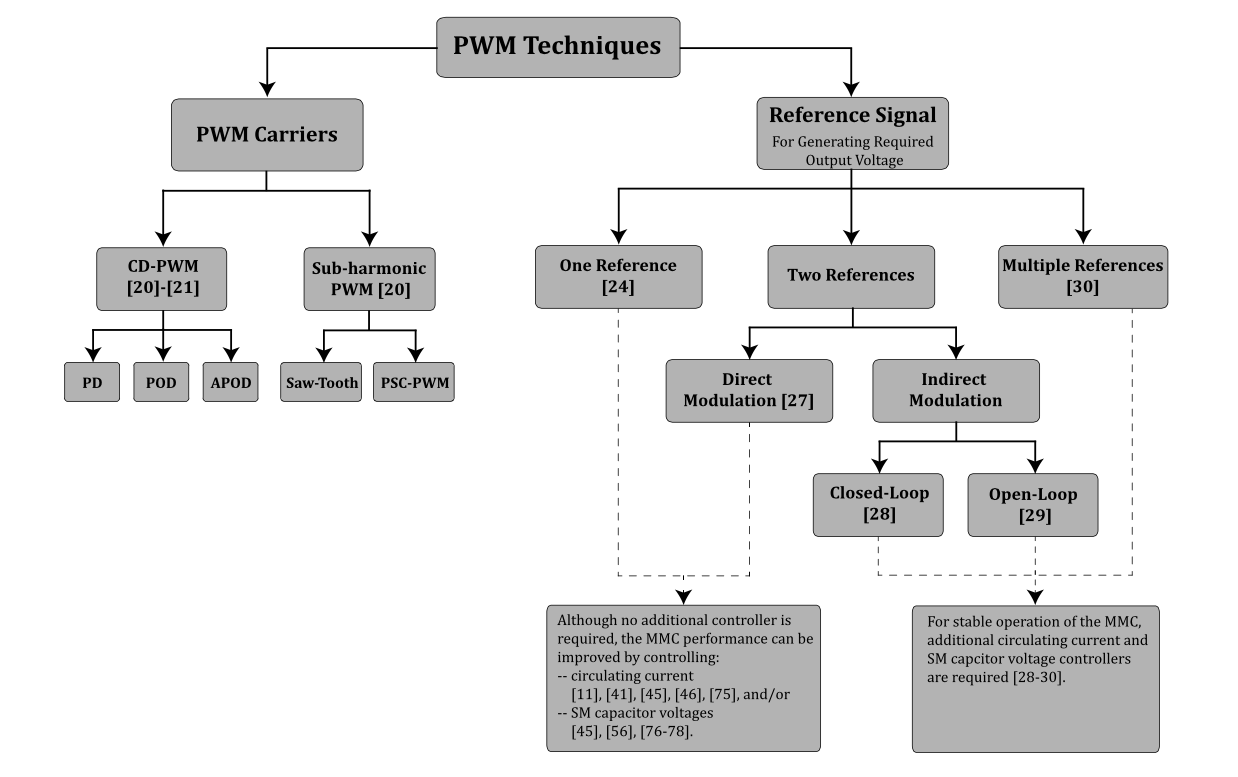
\includegraphics[width=1.05\textwidth]{images/Paper_Fig_5.png}
\setcaptionwidth{\linewidth}
\caption{MMC使用的不同PWM技术概览}
\end{figure}
  
  \subsubsection{SM电容电压平衡}
  
  类似于其他多级换流器技术,MMC需要有功电压平衡策略来平衡和保持SM电容器电压在$V_{dc}/N$。Deng和Zhen在[37]中提出一种电压平衡策略,使用相变换载波PWM(PSC-PWM)来控制MMC桥臂电流中的高频分量。给SM每个桥臂加载合适的PWM脉冲来平衡电容器电压。这增加了控制的简单性并减少了传感器数量。Hagiwara和Akagi在[30]中提出一种电压平衡策略,针对每个SM的闭环控制。在[11]中,开发了一种MMC控制的预测性策略,其中SM电容器电压基于预先定义好的损耗方程平衡。最广泛接受的电压平衡策略是基于排序法(sorting method)[8], [38]-[40]。为了实现基于排序法的电容电压平衡,需要测量和排序SM每一个桥臂的电容器电压。如果$N$个SM对应的桥臂$n_{p,j}(n_n,j)$中上(下)桥臂电压为正,有最低电压的SM被选出开启。结果,对应开启的SM电容器充电,电压升高。如果$N$个SM对应的桥臂$n_{p,j}(n_n,j)$中上(下)桥臂电压为负,有最高电压的SM被选出开启。结果,对应开启的SM电容器放电,电压下降。不考虑上(下)桥臂的电流方向,如果一个桥臂中的Sm被旁路,对应的电容器电压保持不变。尽管排序法保证电容电压平衡在MMC运行要求之下,却在SM中带来了不必要的开关变换。尽管在两个连续控制期中所需运行的SM数保持不变,可能会发生SM的开启或旁路。这个结果不是很理想,因为增加了开关频率相应的增加了能耗,特别是对于高压系统来说。提出/研究的用来减小MMC开关频率的方法主要基于:
  \begin{enumerate}[1)]
  \item 结合相变换载波PWM策略的闭环修正排序法,SM的开启/旁路状态基于电容电压测量[39], [41]。在这种方法中,每个控制环中只有有限数量的SM参加排序,即在每个控制环并基于需要的电压等级,如果需要在每个桥臂中开启(关断)额外的SM,只有关状态(开状态)的Sm需要被考虑排序和开关。
  \item 结合选择性谐波消除PWM技术的开环控制[35]。
  \item 混合平衡策略,结合预测误差排序法和传统的电压排序算法[42]。这种策略基于排序向前一步预测电容电压和其有名值之间的绝对误差来排序。每一个控制期内,有最小预测电压误差的SM被选择开启。
  \item 基频平衡策略,在预先制定的相角下基于传统方法排序。
  \item 一种最优化电容电压平衡策略,排序之前先调整测量之后的SM电容电压。这种策略关注电容电压超过特定电压限制的SM,其他SM的开关状态保持相同。引入保持因子并和关闭状态的电容器电压相乘,这些电容器电压超过电压限增加了在下一个控制环内被开通/旁路的概率。
  \item 一种预测算法来计算和分配储存在SM电容器中的电量[44]。
  \end{enumerate}
  
  \subsubsection{数学模型}
  
\begin{figure}[H]
\centering
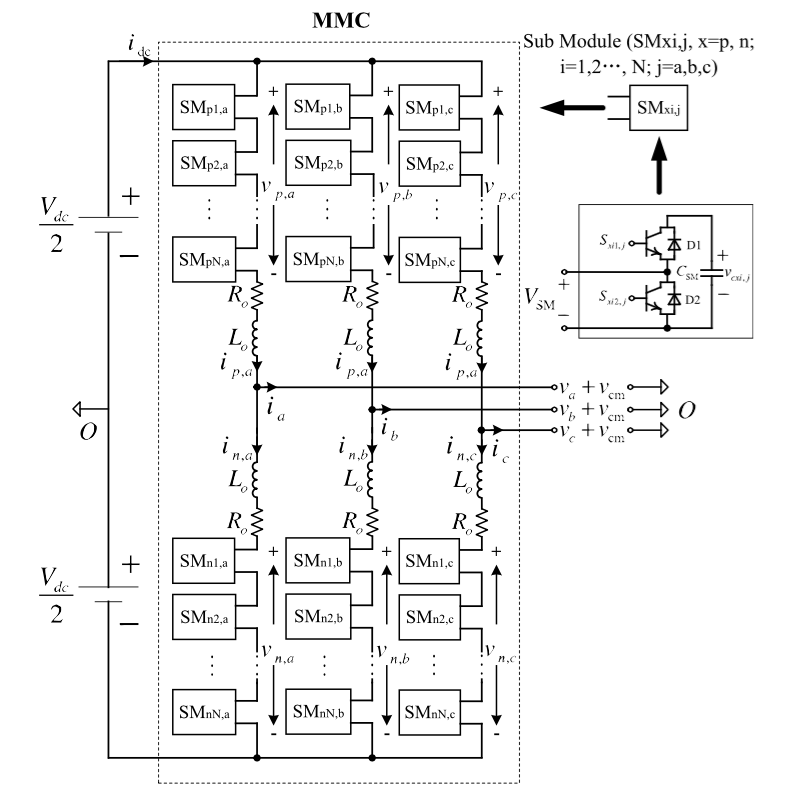
\includegraphics[width=1.05\textwidth]{images/Paper_Fig_6.png}
\setcaptionwidth{\linewidth}
\caption{MMC电路图}
\end{figure}
  图3.5所示为一个基于半桥SM的三相MMC电路图。与图3.1相比,有一个额外的桥臂电阻$R_0$,用来模拟MMC每个桥臂的能耗。
  
  本章建立的MMC数学模型基于文献[8], [11], [45-47]中使用最广泛的模型。
  
  在图3.5中的MMC中,$j$相上下桥臂电流,$j=a, b, c, i.e, i_{p, j}$and$i_{n, j}$表示为:
\begin{align*}
i_{p, j} = \frac{i_{dc}}{3}+i_{circ, j}+\frac{i_j}{2}\tag{4a}\\
i_{n, j} = \frac{i_{dc}}{3}+i_{circ, j}-\frac{i_j}{2}\tag{4b}
\end{align*}

  其中$i_{circ, j}$表示$j$相环路电流,$i_j$是交流侧$j$相电流,$i_{dc}$是直流侧电流。基于(4),环路电流为:
\begin{align*}
i_{circ, j} = \frac{i_{p, j}+i_{n, j}}{2}-\frac{i_{dc}}{3}\tag{5}
\end{align*}

  由$j$相MMC动态行为给出的数学公式为:
\begin{align*}
V_{dc}-v_{p, j} &= L_0\frac{di_{p, j}}{dt}+R_0i_{p, j}+v_j+v_{cm}\tag{6a}\\
V_{dc}-v_{n, j} &= L_0\frac{di_{n, j}}{dt}+R_0i_{n, j}-v_j-v_{cm}\tag{6b}
\end{align*}

  其中$v_{p, j}$和$v_{n, j}$表示MMC$j$相上下桥臂电压,$v_j$和$v_{cm}$分别表示基本和共模电压分量。从(6a)中减去(6b)并从(4)中替换出$i_{p, j}$和$i_{n, j}$,MMC相电压表示为:
\begin{align*}
v_{j}+v_{cm} = \frac{v_{n, j}-v_{p, j}}{2}-\frac{R_0}{2}i_j-\frac{L_0}{2}\frac{di_j}{dt}\tag{7}
\end{align*}

  进一步,将(6a)和(6b)相加并从(5)中减去$i_{circ, j}$,MMC环流内部动态表达为:
\begin{align*}
L_0\frac{di_{circ, j}}{dt}+R_0i_{circ, j} = \frac{V_{dc}}{2}-\frac{v_{n, j}+v_{p, j}}{2}-R_0\frac{i_{dc}}{3}\tag{8}
\end{align*}

  MMC的$j$相上下桥臂电压也可以描述为:
\begin{align*}
v_{p, j} &= n_{p, j}v_{cp, j}\tag{9a}\\
v_{n, j} &= n_{n, j}v_{cn, j}\tag{9b}
\end{align*}
  
  其中$v_{cp, j}$和$v_{cn, j}$分别是上下桥臂独立SM电容器电压。方程(9)基于有功电容器电压策略平衡的假设并保持MMC每个桥臂中所有SM的电容器电压相等,例如$v_{cxi, j, k} = v_{cx, j, k}$对$\forall i\in{1, 2, ..., N}$。将(9)中的$v_{p, j}$和$v_{n, j}$带入(7)和(8),得到下列表达式:
\begin{align*}
v_{j} + v_{cm} &= \frac{n_{n, j}v_{cn, j}-n_{p, j}v_{cp, j}}{2}-\frac{R_0}{2}i_j-\frac{L_0}{2}\frac{di_j}{dt}\tag{10a}\\
L_o\frac{di_{circ, j}}{dt} + R_0i_{circ, j} &= \frac{V_{dc}}{2} - \frac{n_{n, j}v_{cn, j}-n_{p, j}v_{cp, j}}{2} - R_0\frac{i_{dc}}{3}\tag{10b}
\end{align*}

  另外,
\begin{align*}
P_{dc} = P_{ac} + P_{loss} \quad \Rightarrow \quad V_{dc}i_{dc} = \sum_{j = a, b, c}v_ji_j + P_{loss}\tag{11}
\end{align*}
其中$P_{loss}$表示换流器的能耗。

  MMC每一个SM电容电压由每臂的功率建模。每臂的功率由下式给出:
\begin{align*}
p_{p, j} &= v_{p, j}i_{p, j} = n_{p, j}v_{cp, j}i_{p, j}\tag{12a}\\
p_{n, j} &= v_{n, j}i_{n, j} = n_{n, j}v_{cn, j}i_{n, j}\tag{12b}
\end{align*}
  
  MMC每相桥臂上的功率也可以表示为:
\begin{align*}
p_{p, j} = \frac{dW_{p, j}}{dt} &= \frac{d(\frac{N}{2}C_{SM}v^2_{cp, j})}{dt}\\
&= v_{cp, j}NC_{SM}\frac{dv_{cp, j}}{dt}\tag{13a}\\
p_{n, j} = \frac{dW_{n, j}}{dt} &= \frac{d(\frac{N}{2}C_{SM}v^2_{cn, j})}{dt}\\
&= v_{cn, j}NC_{SM}\frac{dv_{cn, j}}{dt}\tag{13b}\\
\end{align*}
其中$C_{SM}$表示SM电容量。基于(12)和(13),每个SM电容器电压波动的动态可以表示为:
\begin{align*}
\frac{dv_{cp, j}}{dt} &= \frac{i_{p, j}}{NC_{SM}}n_{p, j}\\
&= \frac{1}{NC_{SM}}(\frac{i_{dc}}{3} + i_{circ, j} + \frac{i_j}{2})n_{p, j}\tag{14a}\\
\frac{dv_{cn, j}}{dt} &= \frac{i_{n, j}}{NC_{SM}}n_{n, j}\\
&= \frac{1}{NC_{SM}}(\frac{i_{dc}}{3} + i_{circ, j} + \frac{i_j}{2})n_{n, j}\tag{14b}\\
\end{align*}  
  
  (4), (5), (11)和(14)式提供了一个MMC一般化的动态模型,可以用于控制目的。类似于MMC的这种一般化动态模型,参考文献[27]和[28]将每个桥臂中电容电压的累加组成的MMC动态模型看成是一个静态变量,而不是独立的SM电容电压。

  \subsubsection{MMC设计限制}
  MMC的设计包括选择电容、电感和SM的数量,基于一些性能指标包括桥臂电流波动、短路电流、电容电压波动、可靠性和能耗。
  \begin{enumerate}[1)]
  \item \emph{电容电感选型:}桥臂电感$L_0$作为滤波器来减小桥臂电流中的高频谐波同时也限制了直流侧短路电流。因此,桥臂电感的大小取决于滤波选择和短路电流限制[5], [51], [52]。
  
  SM电容的选型基于对大小/能耗和电压震荡的权衡。在很大范围的运行环境中,SM电容电压震荡在[55]-[59]中得到分析。对于SM电容电压$\delta v_{c, pp}$考虑一个许可的峰峰谐波等级,基于[55]的元电容取决于:
\begin{align*}
C_{SM} = \frac{P}{3NmV_c\delta c_{c, pp}\omega cos\theta}(1-(\frac{mcos\theta}{2})^2)^{\frac{3}{2}}\tag{15}
\end{align*}
其中$C_{SM}$是SM电容,$P$是有功功率,$V_c$是SM电容器的标么电压,$m$是调节指数,而$cos\theta$是功率因数。

  基于存储能量和功率流动的关系,[61]提出一个SM电容器选型方法。
  \item \emph{功率损耗计算:}相比于二级VSC系统,半导体损耗大于1\%[13],MMC的半导体损耗可以潜在地降低到低于1\%。
  
  主要有两种方法来评估MMC的半导体损耗。第一种取决于仿真模型和实时仿真数据[40], [63]-[67]。尽管这种方法的计算压力很大,却可以提供精确的结果而不用考虑模块化/控制策略,电压等级和SM电路拓扑。[62]和[63]介绍的另一种方法,基于分析性模型可以潜在地降低计算时间。可是,保证精度方面是一个挑战因为这种方法基于理想假设和特殊的模块化/控制策略。
  \item \emph{可靠性:}MMC因为其模块化的结构,可以提升冗余SM结构中的容错限[12], [68],进而提升其可靠性。可是,在特定的容错限之下,控制硬件限制了换流器的稳定性。
  \end{enumerate}
  
  \subsubsection{环路电流控制}
  
  流经MMC三相桥臂的环路电流源自三相桥臂中的电压差异[53], [70]并且包含频率是基频两倍的负序分量[70]。环路电流对于交流侧电压电流没有任何影响。可是,如果不正确地控制,他们会增加相电流的峰值结果将增加换流器的能耗和SM电容电压的震荡大小。环路电流在[70]-[72]中被建模和分析。[71提出一种环路电流模型基于控制环路电流为电流控制电压源。这可以接着被用于控制电压来降低环路电流分量的影响。
  
  为了控制环路电流,文献[11], [28]-[30], [41], [45], [46], [57], [73], [74]中提出了各种各样的技术。[28]-[30]中的间接建模技术在前述章节中已经介绍。Harmefors等人使用有功电阻(合适的控制器)来控制环路电流,包括对桥臂电阻的估计。基于双线频$acb-dp$变压器,Tu等人[41]通过控制他们一对PI控制器的的$dp$部分来减小环路电流。Debnath和Saeedifard[45]等人致力于降低通过比例共鸣(PR)控制器的环路电流的交流分量。Yang[57]等人提出一种改进的开关函数来消除用于STATic和COMpensator(STATCOM)中的MMC环路电流。[11]提出一种基于模型的预测控制(MPC)来降低环路电流分量。主要缺点在于计算量大,尤其对于有大量SM的MMC来说。
  
  \subsubsection{SM电容电压震荡消除技术}
  
  [55]深入研究了SM电容电压震荡, [57]-[59]主要研究基频和二次谐波分量。基于桥臂功率,[76]提出使用合适的二次谐波分量来降低SM电容电压的震荡大小。使用二次和四次谐波分量[56]中的方法最优化了每个桥臂中的能量变化。Debnath和Saeedifard[45]提出一种闭环控制策略来减小电容电压波动的二次谐波分量并且数学地证明了所提出的方法简介见底了电容电压的震荡大小。
  
  Engel和Doncker[56]提出最优化方法通过保持桥臂电流的rms值来降低电容电压波动,进而限制了换流器的功率损失。
  
  除了SM电容电压波动的减小策略,文献[49]和[79]变形电容电压波动来最大化运行区域(有功率极限定义)。
  
  \subsubsection{SM电容预充电和启动过程}
  
  MMC启动时,在正常工作之前需要提前充电到相等的特定电压等级。为了减小冲击电流和启动时间,最好是一种快速平滑启动。[55], [80]-[86]从去能量化的角度研究了MMC中SM电容器的预充电和启动过程。启动过程经两步进行:1)分别充电直流侧电容器和经过二极管桥整流器的SM电容器至$V_{dc}$和${\frac{V_{dc}}{2N}}$,假设所有SM电容器插入直流侧并且涌入电流被交流侧的串联电阻限制,2)旁路交流测电阻接着从$2N$到$N$逐渐减少开通SM的数量,进而让电容从$\frac{V_{dc}}{2N}$到$\frac{V_{dc}}{N}$。
  
  \subsection{特殊情况下MMC的运行}
  
  \subsubsection{非平衡电网条件}
  
  建模和仿真MMC的主要技术文献假设系统处于平衡状态[1]-[7], [9], [10], [12]。非平衡条件下MMC的控制在文献[8], [9], [87]-[89]中有讨论。在非平衡电网条件下,主要的控制目标是:i)通过限制负序分量来平衡交流侧电压,ii)调节电网直流总线电压,iii)控制环路电流和SM电容器电压。
  
  Saeedifard和Iravani[8]提出了一种普遍的PWM策略来在非平衡电网条件下控制MMC,这种情况下,MMC动态可以被视为两个解耦的子系统,正序和负序子系统;每个子系统可以被分别控制。
  
  Tu等人[87]提出一种直流电压波动限制的控制器来去除非平衡电网条件下直流侧零序分量并保持电网直流总线电压恒定。可是,在非平衡电网电压条件下,在实际功率器件中有双线频率波动。Guan和Xu在[9]中提出零序交流电压控制器,和正负序交流电压控制器,来在非平衡电网条件下运行MMC-HVDC系统通过/不通过接口变压器。
  
  \subsubsection{容错运行}
  
  如前面所提到的,MMC的模块化设计提高了其冗余和容错。在任何原件/SM失效的前提下,失效的SM需要被检测出来并旁路。当一个开环错误出现时,MMC的输出电压和电流紊乱。进一步,失效的SM电容器电压升高,导致更大的破坏。
  
  \subsection{应用}
  
\begin{figure}[H]
\begin{minipage}[t]{0.5\linewidth}
\centering
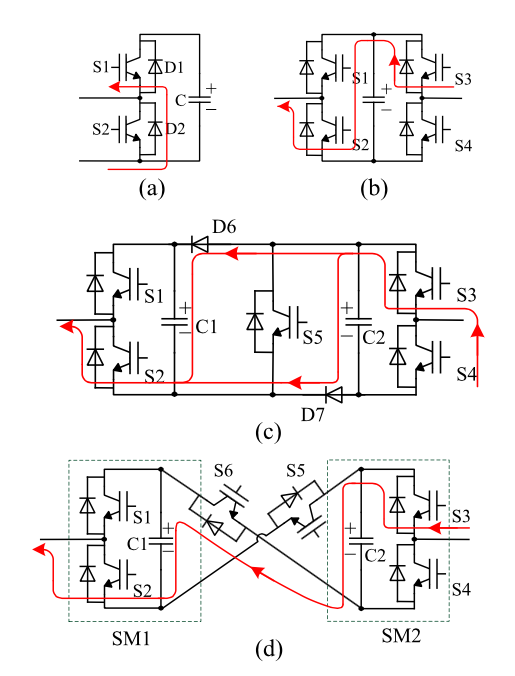
\includegraphics[width=3.2in]{images/Paper_Fig_7.png}
\setcaptionwidth{2.5in}
\caption{直流侧短路错误电流路径:\quad (a) \quad 半桥;\quad (b) \quad 全桥;\quad (c) \quad 双钳制;\quad (d) \quad 五级跨接SM}
\end{minipage}%
\begin{minipage}[t]{0.5\linewidth}
\centering
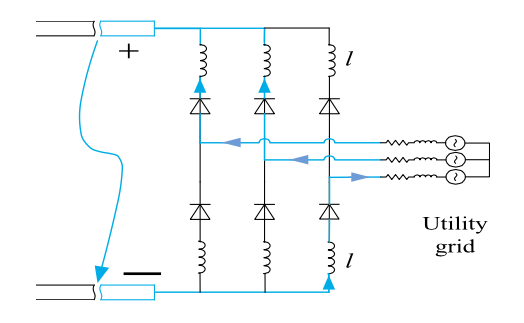
\includegraphics[width=3.2in]{images/Paper_Fig_8.png}
\setcaptionwidth{2.5in}
\caption{直流短路时MMC系统的等效电路}
\end{minipage}
\end{figure}  
  
  \subsubsection{HVDC系统}
  
  MMC最初是为了HVDC系统而提出,变成了HVDC系统最可靠的VSC形式。采用传统半桥SM的MMC-HVDC系统的一个主要挑战之一是缺少直流侧电流错误处理能力。这个问题非常严重,尤其是对于没有过载能力的HVDC系统来说。现有的干预和处理MMC-HVDC系统直流侧短路故障的方法总结如下:
  \begin{enumerate}[1)]
  \item 打开交流侧CB。这种方案并不是很快速因为它需要几个循环,比如两到三个循环。结果是,组成非控制整流器的MMC惯性二极管需要忍受几个循环高故障电流。
  \item 采用直流侧CB。尽管用于HVDC的固态直流CB怎年来得到开发,但这项技术并不是很成熟费用也比较高。
  \item 在HVDC换流器结构中嵌入直流故障处理能力。
  \end{enumerate}
  
  \subsubsection{变速伺服}
  
  MMC在中压变速伺服中的应用比其他多级换流器例如NPC和串联H桥换流器有更大的优势。可是,这种应用有其自身独有的控制挑战。主要的挑战在于在低频情况下SM电容器电压有很大的波动量。
  
  SM电容电压的峰峰波动量由下式给出[83]:
\begin{align*}
\delta v_{c, pp} = \frac{I_0}{2C_{SM}\omega}(1-(\frac{mcos\theta}{2})^2)^{\frac{3}{2}}\tag{16}
\end{align*}
其中$i_{circ, j}\approx 0$,$I_0$是交流侧相电流$(i_j)$大小,$m$是$m_j$的幅值,$\omega$是交流侧相角频率,$\theta$是交流侧功率因数角。如式(6)所示,SM电容电压的波动幅值反比例于交流频率并且正比例与交流侧相电流幅值。结果,在恒转矩应用中,SM电容器电压的波动幅值在低频时变得很大。这种情况在正交转矩应用时不那么明显因为电流幅值正比于频率。因此,有必要减小SM电容器电压的低频波动分量当MMC应用在变频恒转矩情况下时。

  \subsubsection{动态制动斩波器}
  
  在很多应用中,直流制动斩波器需要吸收和分解能量。一个例子是离岸风电场中的基于MMC的HVDC变换系统。因为MMC-HVDC末端无法接收风电场的功率,例如按上电网的非永久性故障,电网无法忍受离岸电站的任何故障。因此,如图3.8所示,岸上电站需要吸收和分解风电场的功率而在出现故障时不干扰风电场的运行。这就需要在VSC-HVDC换流站离岸直流侧安装由如图3.8所示的制动电阻来实现。
  
  另外,图3.9所示为串联连接SM的模块化设计,使模块化斩波器能够满足最小费用和空间的情况下被安装到岸上。
\begin{figure}[H]
\begin{minipage}[t]{0.5\linewidth}
\centering
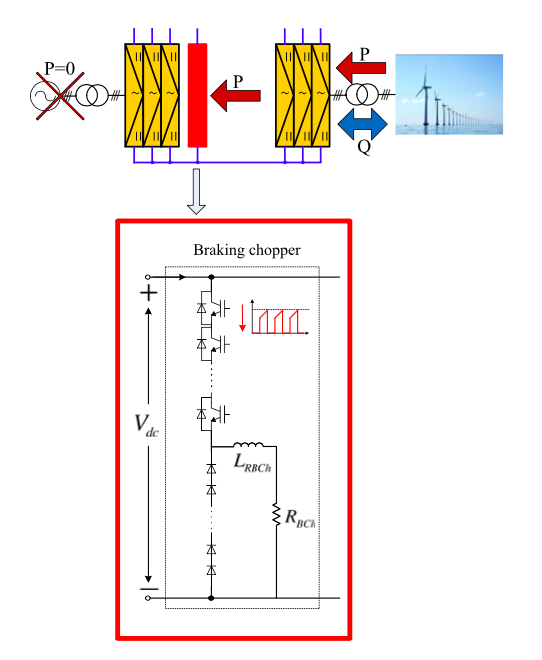
\includegraphics[width=3.2in]{images/Paper_Fig_9.png}
\setcaptionwidth{2.5in}
\caption{传统制动斩波器电路}
\end{minipage}%
\begin{minipage}[t]{0.5\linewidth}
\centering
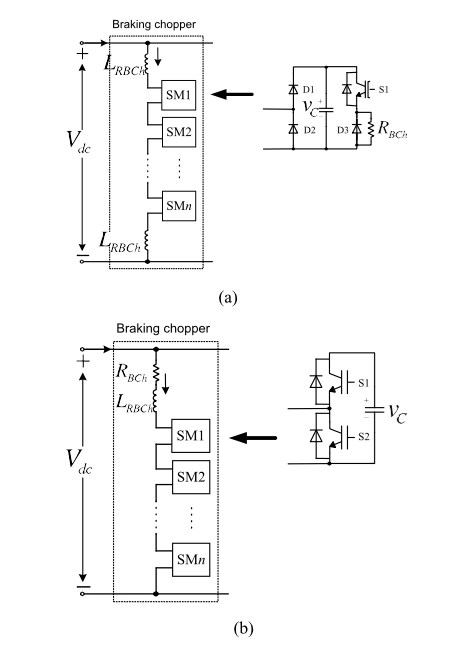
\includegraphics[width=3.2in]{images/Paper_Fig_10.png}
\setcaptionwidth{2.5in}
\caption{基于MMC概念的模块化制动斩波器}
\end{minipage}
\end{figure} 

  \subsection{结论}
  
  MMC的主要特征,例如其模块化和可测量性使其理论上满足任何电压等级的需求,有非常好的谐波性能和很高的效率。在过去几年中,对各种中/高压电压/功率系统和包括HVDC转换系统、FACTS、中压变速伺服和中/高压dc-dc换流器在内的工业应用,MMC变成了一个热点问题。
  
  对电力系统应用来说,例如HVDC系统和FACTS,MMC有一定的成熟度,并且似乎是最主流的技术,因为很多MMC-HVDC系统和STATCOMs被成功地完成和安装起来。
  
  对于中压变速伺服,有关MMC的运行和控制未来还有很多发展空间,尤其是在常转速低速的情况下。需要注意的一个主要问题是在低频情况下减小电容器电压波动的大小同时不牺牲换流器效率,因此需要在换流器大小/容量/费用和效率之间做一个权衡。
  
  源自MMC拓扑的一类模块化舵机dc-dc换流器的引入打开了中/高压dc-dc换流器领域研究和发展的一个新方向。为了更好的应用在各种应用中去,需要有高压换流器比率、高效率和器件压力较小的的高级模块化策略。
  
  随着大量出现的源自MMC的换流器拓扑和应用,可以得出结论,新的模块化和控制策略的发展会是未来MMC应用的主要推动力。
  
  
  
  %开题报告
  \chapter{开题报告}

\section{项目研究目的}
现在电力系统常用的数据格式是基于BPA文本文件,其缺陷是不易于实现自定义等高级操作,在研究新能源或新设备并网问题时,需要在现有的大电网模型基础上建立新元件模型,但 BPA 不能修改和自定义元件模型。相比之下,DIgSILENT 具有可靠灵活的系统建模能力,该软件不仅包含了其他电力系统仿真软件中的潮流、短路、机电暂态、电磁暂态等分析功能,还具有很多独特而实用的优点。它是以图形化操作和数据管理技术为支撑,便于调试和结果分析;具有风力发电、光伏发电等元件模型,也可由用户自定义各种与那件模型。

针对电力系统不同的问题,采用较优的电力系统商业软件,可以使得科研分析等工作具有事半功倍的效果。因此需要数据转换程序,以便能够选择需要的仿真软件进行仿真。

\section{研究内容和研究步骤}
研究内容主要分为以下几个方面:

\begin{itemize}
\item 复习潮流计算中所使用的主要数据类型和数据格式。
\item 学习BPA的主要功能和数据格式,BPA 数据是基于卡片格式的,主要的潮流数据卡片可以分为五类,分别为区域控制数据卡、节点数据卡、支路数据卡、变压器卡及数据修改卡。进而学习DIgSILENT的数据格式和相关操作,DIgSILENT 采用的是分层的面向对象的数据库, 潮流数据填入各个代表元件的图形中储存为对象。
\item 阅读、学习由BPA到PSS/E的实现程序和董炜学长编写的BPA到DIgSILENT转换程序,在这个过程中形成自己对BPA到DIgSILENT程序转换的思路,着重理解相关参数的对应和转化,发现方法。
\item 完成程序的编写,对比分析几个软件的潮流计算结果。
\item 带入相关的算例进行测试,对比BPA和DIgSILENT的动态计算结果。
\end{itemize}

\section{程序的大体思路}

DIgSILENT自带的DPL 程序在处理以下操作中有较明显的优势: (1)实现 DIgSILENT 内部数据的导入和导出;(2) 访问或更改的 DIgSILENT 内部对象。

DPL的缺点是:不能像Python语言那样实现比较灵活和通用的功能,DPL 的开发环境不能像Python语言那样提供调试功能。因此,DPL适用于程序代码较短的功能,并不适于开发大型或复杂的功能。

因此,将DPL实现困难的部分使用Python实现,DPL易于实现的功能还是使用DPL完成,用Python整体控制转换程序的运行。主要有以下重点:(1)使用Python调用DPL程序;(2)DPL程序执行结束后,及时通知Python主程序,以便主程序执行下一步功能。

BPA 模型导入 DIgSILENT 需要以下步骤:
  \begin{enumerate}[1)]
  \item 检查 DIgSILENT 中创建的元件模型名称与 BPA 中的是否一致,给用户错误提示,直到所有错误都修改后才能继续下面步骤。可先从 DIgSILENT 导出包含电网模型的 DGS 文件,解析出元件模型名称和元件间连接关系;然后解析出 BPA 模型文件中的相关数据;最后进行对比分析。
  \item 检查 DIgSILENT 中创建的电网拓扑连接与 BPA 中的是否一致。也是通过解析对比 DGS 文件和 BPA 模型文件实现。
  \item 按照自定义的命名规则,给 DIgSILENT 中所有元件的 Foreign Key 属性定义并填入唯一的值。
  \item 将 BPA 数据文件转换为 DGS 文件。
  \item 在 DIgSILENT 中导入 DGS 文件,实现批量给元件模型赋值。
  \end{enumerate}

\section{论文的主要内容和进度安排}

本文的主要内容是通过文献资料的阅读整理,学习数据转换的基础理论知识,了解有关的常规算法以及新提出的改进算法,研究这些算法的理论并且对目前常用的算法进行收集整理,分析各种算法的优缺点以及适用条件。认识并熟悉BPA和DIgSILENT的基本使用技巧,了解他们的数据格式,编程语言,并能有一定应用。

进度安排

3月23日-4月5日:进行文献资料的阅读学习,学习软件编程语言和仿真软件,研究董炜学长的Python程序,熟悉软件使用;

4月6日-4月19日:进行程序的开发和调试;

4月20日-5月3日:结合算例对比程序运行结果,改进程序;

5月4日-结题:完成毕业论文的撰写。



  
  %Python
  \chapter{DIgSILENT的Python接口简介}

\section{Python脚本语言的优势}

本章主要介绍在\emph{PowerFactory}中整合Python脚本语言的接口,并解释了在DIgSILENT中开发Python脚本的相关步骤。在\emph{PowerFactory}中,Python脚本语言主要实现以下功能:

\begin{itemize}
\item 任务自动化执行
\item 创建用户自定义的运算指令
\item 将\emph{PowerFactory}整合到其他应用程序之中
\end{itemize}

DIgSILENT自带的DPL程序在可以快速实现 DIgSILENT 内部数据的导入和导出,并且易于访问或更改DIgSILENT内部对象。但是,DPL存在以下明显缺点:

\begin{itemize}
\item DPL不能像Python语言那样实现比较灵活和通用的功能
\item DPL 的开发环境不能像Python语言那样提供调试功能
\end{itemize}

因此,DPL适用于程序代码较短的功能,并不适于开发大型或复杂的功能。相比于DPL,Python脚本语言有以下明显的优势:

\begin{itemize}
\item Python适用性强,并不是为DIgSILENT专门设计,属于高级编程语言
\item 语法简单,逻辑清晰,程序可读性强
\item 免费,适用于开源协议
\item 用途极其广泛
\item 有大量的标准运行库和第三方接口模块

	\begin{description}
	\item[-] 对外部数据库和类似于Microsoft Office应用程序的接口
	\item[-] 网络互联服务等等
	\end{description}

\end{itemize}

对Python的整合使得\emph{PowerFactory}可以实现以上提到的种种优势,要在\emph{PowerFactory}中使用Python,需要遵循以下步骤:

\begin{enumerate}
\item 安装Python脚本解释器
\item 使用\emph{PowerFactory}中的Python模块\emph{'power factory.pyd'}编写Python脚本程序
\item 通过\emph{PowerFactory}中的Python命令对象(\emph{ComPython})执行Python脚本
\end{enumerate}

\section{\emph{PowerFactory}中的Python模块}

\begin{figure}[H]
\centering
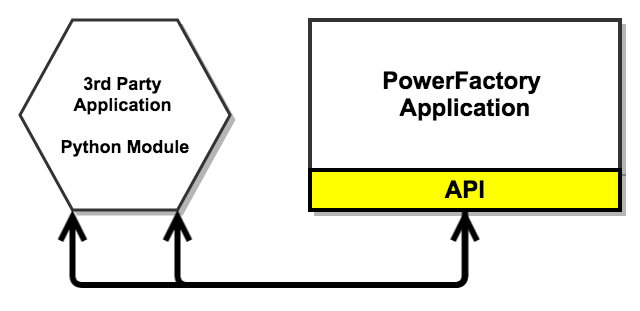
\includegraphics[width=1.05\textwidth]{images/Paper_Fig_13.png}
\setcaptionwidth{\linewidth}
\caption{Python Module 通过API与\emph{PowerFactory}交互示意图}
\end{figure}

如图4.2所示,Python脚本主要通过一个和\emph{PowerFactory API}交互的动态Python模块(\emph{'power factory.pyd'})来实现\emph{PowerFactory}的相关功能。这种方法使得Python脚本可以使用\emph{PowerFactory}中的大量数据,包括:

\begin{itemize}
\item 所有对象
\item 所有属性(元件数据,类型数据,结果)
\item 所有命令(潮流计算等等)
\item 大部分特殊内建函数(DPL函数)
\end{itemize}

导入这个动态模块的Python脚本可以通过\emph{PowerFactory}内部命令行对象\emph{ComPython}来运行,或者通过外部引擎使用。

\section{Python命令行对象(\emph{ComPython})}

Python命令行对象(\emph{ComPython})如图4.2将Python脚本链接到\emph{PowerFactory}。它仅仅保存文件的路径而不是具体文件。

\begin{figure}[H]
\centering
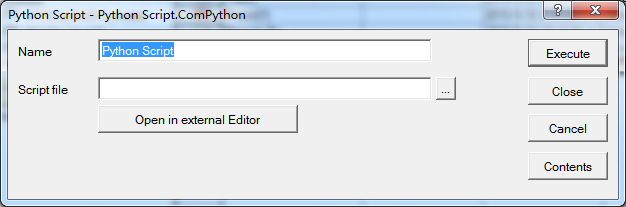
\includegraphics[width=1.05\textwidth]{images/Paper_Fig_15.png}
\setcaptionwidth{\linewidth}
\caption{Python命令行对象(\emph{ComPython})对话框}
\end{figure}

脚本可以通过点击\textbf{Execute}按键来执行,可以通过点击\textbf{Open in external Editor}来比编辑脚本,脚本的编码需采用UTF-8编码格式。

要新建一个Python命令对象,需点击\emph{New Object}按钮,并选择如图4.3所示\emph{DPL Command and more}选项,在下拉菜单中选择\emph{Python Script}。

\begin{figure}[H]
\centering
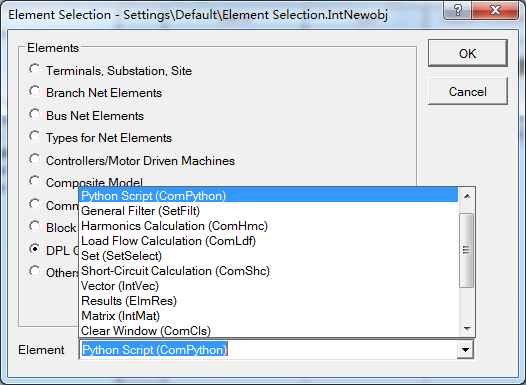
\includegraphics[width=1.05\textwidth]{images/Paper_Fig_14.png}
\setcaptionwidth{\linewidth}
\caption{新建一个Python命令行对象(\emph{ComPython})}
\end{figure}

\section{调试Python脚本}

与其他Python脚本一样,\emph{PowerFactory}也可以通过特殊应用程序来调试。

\subsection{准备条件}

推荐使用Eclipse IDE来调试Python甲苯,需要安装Python插件\emph{PyDev}。

\begin{enumerate}
\item 从\emph{www.eclipse.org/downloads/}安装Eclipse Standard
\item 点击\emph{help}菜单中的\emph{"Install New Software ..."},添加目录\emph{http://pydev.org/updates}并安装\emph{PyDev}
\end{enumerate}

\subsection{为\emph{PowerFactory}调试Python脚本}

如下所示是一个通过\emph{PyDev}远程调试Python脚本的介绍。

\begin{enumerate}
\item 启动Eclipse并打开\emph{Debug}视图
\item 通过点击\emph{PyDev}菜单中的\emph{"Start Debug Server ..."}启动远程调试服务
\item 准备待调试的Python脚本:

	\begin{description}
	\item[-] 在\emph{sys.path}中添加\emph{"pydevd.py"}
	\item[-] 导入PyDev调试模块\emph{"pydevd"}
	\item[-] 通过启动\emph{pydevd.settrace()}开始调试
	\end{description}
	
Example:

\begin{minted}[fontsize = \footnotesize, frame=lines, framesep=2mm, baselinestretch=0.7]{python}
#prepare debug
import sys
sys.path.append \
("C:\\Program Files\\eclipse\\plugins\\org.python.pydev\\pysrc")
import pydevd
#start debug
pydevd.settrace()
\end{minted}

	
\item 运行该脚本的Python命令行对象(\emph{ComPython})
\item 进入Eclipse使用远程调试服务调试

\end{enumerate}




%==============================================================
%这也是个不需要自己修改的部分。

  \backmatter %结束章节自动编号

  %参考文献
  \addcontentsline{toc}{chapter}{参考文献} % 解决目录中没有相应的参考文献的条目问题
  \chaptermark{参考文献}

%==============================================================

  \bibliography{data/zjubib}

  %致谢
  %致谢
\chapter*{\centerline{致\quad 谢}}
\chaptermark{致谢}
\addcontentsline{toc}{chapter}{致谢}

\vspace{2em}

感谢电气工程学院四年来对我的辛苦培育,特别感谢老师们四年来对我无微不至的关怀和指导让我在大学这四年来学到很东西。在此,我还要感谢在班里同学和朋友,感谢你们在我遇到困难的时候帮助我,给我支持和鼓励,感谢你们。

特别感谢我的导师甘德强老师和师兄董炜学长,在程序开发中给予我悉心指导,从开发到结束中过程遇到很多困难都是他给我鼓励与指引,使我能够克服重重困难,将程序完成,在此谨向甘老师和董师兄致以诚挚的谢意和崇高的敬意。谢谢!
  %附录
  \chapter*{附\quad 录}
\chaptermark{附录}
\addcontentsline{toc}{chapter}{附录} 


  %任务书
  %任务书
\chapter*{\centerline{\stxingkai\erhao 本科生毕业论文(设计)任务书}}
\thispagestyle{empty}

\vspace{2em}

{\stfangsong\xiaosi\bf
一、\;题目:\;\uline{\hfill\hspace{4mm}}

二、\;指导教师对毕业论文(设计)的进度安排及任务要求:
\vspace{4cm}

\begin{flushright}
起讫日期 200 \quad 年 \quad 月 \quad 日 至 200 \quad 年 \quad 月 \quad 日\\
指导教师(签名)\;\underline{\hspace{4em}} \quad 职称\;\underline{\hspace{4em}}
\end{flushright}

三、\;系或研究所审核意见:
\vspace{4cm}
\begin{flushright}
负责人(签名)\underline{\hspace{4em}}\\
\quad 年 \quad 月 \quad 日
\end{flushright}
}

  %考核
  %考核
\chapter*{\centerline{\stfangsong\xiaoer 毕~业~论~文~(设计)~考~核}}
\thispagestyle{empty}

\vspace{2em}

{\stfangsong\sihao\bf
一、\;指导教师对毕业论文(设计)的评语:
\vspace{4cm}

\begin{flushright}
    指导教师(签名)\;\underline{\hspace{4em}}\\
    年\quad 月\quad 日
\end{flushright}

二、\;答辩小组对毕业论文(设计)的答辩评语及总评成绩:
\vspace{4cm}

{\songti\xiaosi
\begin{tabular}{|c|c|c|c|c|c|}
    \hline
    成绩比例 & \parbox[t]{4em}{文献综述\\[-3.5em]占(10\%)} & 
               \parbox[t]{4em}{开题报告\\[-3.5em]占(20\%)} & 
               \parbox[t]{4em}{外文翻译\\[-3.5em]占(10\%)} &
               \parbox[t]{7em}{毕业论文(设计)\\[-3.5em]质量及答辩\\[-3.5em]占(60\%)} & 
               总评成绩 \\
    \hline
    分值 & & & & & \\
    \hline
\end{tabular}
}

\begin{flushright}
    答辩小组负责人(签名)\;\underline{\hspace{4em}}\\
    年 \quad 月 \quad 日
\end{flushright}
}


%==============================================================
%==============================================================
\end{document}
